% THIS DOCUMENT IS FOLLOWS THE VOLERE TEMPLATE BY Suzanne Robertson and James Robertson
% ONLY THE SECTION HEADINGS ARE PROVIDED
%
% Initial draft from https://github.com/Dieblich/volere
%
% Risks are removed because they are covered by the Hazard Analysis
\documentclass[12pt]{article}

\usepackage[round]{natbib}
\usepackage[letterpaper, portrait, margin=1in]{geometry}
\usepackage{booktabs}
\usepackage{siunitx}
\usepackage{tabularx}
\usepackage[dvipsnames]{xcolor}
\usepackage{hyperref}
\usepackage{enumitem}
\usepackage{graphicx}
\hypersetup{
    bookmarks=true,         % show bookmarks bar?
      colorlinks=true,      % false: boxed links; true: colored links
    linkcolor=red,          % color of internal links (change box color with linkbordercolor)
    citecolor=green,        % color of links to bibliography
    filecolor=magenta,      % color of file links
    urlcolor=cyan           % color of external links
}

\newcommand{\lips}{\textit{Insert your content here.}}

%% Comments

\usepackage{color}

\newif\ifcomments\commentstrue %displays comments
%\newif\ifcomments\commentsfalse %so that comments do not display

\ifcomments
\newcommand{\authornote}[3]{\textcolor{#1}{[#3 ---#2]}}
\newcommand{\todo}[1]{\textcolor{red}{[TODO: #1]}}
\else
\newcommand{\authornote}[3]{}
\newcommand{\todo}[1]{}
\fi

\newcommand{\wss}[1]{\authornote{blue}{SS}{#1}} 
\newcommand{\plt}[1]{\authornote{magenta}{TPLT}{#1}} %For explanation of the template
\newcommand{\an}[1]{\authornote{cyan}{Author}{#1}}

%% Common Parts

\newcommand{\progname}{Software Engineering} % PUT YOUR PROGRAM NAME HERE
\newcommand{\authname}{Team 6, EcoOptimizers
\\ Nivetha Kuruparan
\\ Sevhena Walker
\\ Tanveer Brar
\\ Mya Hussain
\\ Ayushi Amin} % AUTHOR NAMES                  

\usepackage{hyperref}
    \hypersetup{colorlinks=true, linkcolor=blue, citecolor=blue, filecolor=blue,
                urlcolor=blue, unicode=false}
    \urlstyle{same}
                                


\begin{document}

\pagenumbering{roman}

\title{Software Requirements Specification for \progname: subtitle describing software} 
\author{\authname}
\date{\today}
	
\maketitle
\thispagestyle{empty}

~\newpage

\tableofcontents

~\newpage

\section*{Revision History}

\begin{tabularx}{\textwidth}{p{3cm}p{2cm}X}
\toprule {\textbf{Date}} & {\textbf{Version}} & {\textbf{Notes}}\\
\midrule
Date 1 & 1.0 & Notes\\
Date 2 & 1.1 & Notes\\
\bottomrule
\end{tabularx}

~\\

~\newpage
\pagenumbering{arabic}

\section{Purpose of the Project}
\subsection{User Business}
The Information and Communications Technology (ICT) sector, an essential component of the global economy, is 
responsible for 2-4\% of global CO2 emissions today, with projections suggesting this could rise to 14\% by 
2040 ~\citep{BelkhirAndElmeligi2018}. To meet sustainability goals, including a 72\% reduction in CO2 
emissions by 2040 ~\citep{FreitagAndBernersLee2021}, this sector must find ways to improve energy efficiency.

One area of concern is the energy consumption of software systems. However, for software engineers, it is 
not practical for them to focus on optimizing energy consumption while developing complex programs. 
Instead, supporting tools and technologies are needed to assist in improving energy efficiency without 
altering the intended behaviour of the software.

This project aims to tackle Python, a popular but energy-inefficient programming language. Python consumes 
significantly more energy compared to more efficient languages like C and Rust—over 70 times more energy, 
on average, for similar tasks ~\citep{PereiraEtAl2017}. The project's goal is to develop tools to reduce 
Python's energy consumption through automated refactoring. While this will not solve the entire problem of 
the carbon footprint associated with the software, it is a step towards more energy-efficient practices in 
the software development process.

\subsection{Goals of the Project}
\noindent \textbf{Purpose}: The purpose of this project is to provide software engineers with tools to optimize 
the energy efficiency of Python programs by automating refactoring suggestions, while still allowing 
users to review and decide whether or not to apply the changes.

\noindent \textbf{Advantage}: By reducing the energy consumption of Python programs, this project will 
contribute to the broader effort of decreasing the carbon footprint of software development, supporting 
the ICT sector's goal of reducing CO2 emissions by 72\% by 2040 ~\citep{FreitagAndBernersLee2021}.

\noindent \textbf{Measurement}: The project's success can be measured by the reduction in energy usage 
achieved after applying the refactorings. Benchmarks will compare the energy consumption of original 
and refactored code, to achieve a measurable percentage reduction in energy consumption. The user's 
ability to make informed choices about whether to apply refactorings will also be evaluated through 
user feedback.

\section{Stakeholders}
\subsection{Client}
The client of this project is \textbf{Dr. Istvan David} from McMaster's Department of Computing and Software. As the project supervisor, his role is to guide the development team with his technical and domain expertise. As the client, he sets the product's requirements and will be involved throughout its development. 
\subsection{Customer}
The customers of this product are all the \textbf{software developers} that use it to improve the energy efficiency of their codebase. They will be the primary users of the product and, therefore, will offer critical feedback on its effectiveness. Suggestions for improvement and/or additional features may come from this stakeholder. 

\subsection{Other Stakeholders}
\subsubsection*{\textcolor{Maroon}{Project Managers}}
They oversee project operations and focus on reducing energy costs associated with large-scale or cloud-hosted applications. They might leverage the refactoring library to reduce operational costs and achieve business sustainability goals.

\subsubsection*{\textcolor{Maroon}{Business Sustainability Teams}}
This stakeholder is responsible for reducing their company's environmental footprint by analyzing its energy emissions. They will use the energy efficiency metrics provided by the refactoring library to improve environmental sustainability practices within their organization.

\subsubsection*{\textcolor{Maroon}{End Users}}
End users refer to the users of software that uses the product in its development. They will indirectly reap benefits from these applications that have been optimised using the refactoring library. They might experience more responsive, efficient software, particularly in mobile or embedded environments where battery life is a key concern. They have no involvement in the development of the product. 

\subsubsection*{\textcolor{Maroon}{Regulatory Bodies}}
This stakeholder is responsible for establishing regulations governing energy consumption and sustainability standards. They can promote the adoption of energy-efficient software practices and potentially certify tools that meet regulatory standards. 

\subsection{Hands-On Users of the Project}
\subsubsection*{\textcolor{Maroon}{Software Developers}}
\begin{itemize}
  \item \textbf{User Role}: Integrate library into codebase, provide tests to check refactoring against original functionality

  \item \textbf{Subject Matter Experience}: Journeyman to Master
  
  \item \textbf{Technological Experience}: Journeyman to Master
  
  \item \textbf{Attitude toward technology}: Varies (conservative to positive)
  
  \item \textbf{Physical location}: Remote (at home), in-person (work office) or hybrid
\end{itemize}

\subsubsection*{\textcolor{Maroon}{Business Sustainability Teams}}
\begin{itemize}
  \item \textbf{User Role}: Access metrics provided by library

  \item \textbf{Subject Matter Experience}: Journeyman

  \item \textbf{Technological Experience}: Novice to Journeyman
  
  \item \textbf{Attitude toward technology}: Neutral to positive

\end{itemize}

\subsection{Personas}

\textbf{Persona 1} \\
Raven Reyes, a 34-year-old senior software developer, has over a decade of experience in backend development. Now working at a SaaS company focused on sustainability, Raven faces the challenge of reducing the energy consumption of their software. Manually refactoring code is time-consuming, especially when trying to pinpoint which parts of the code are draining the most energy. With tight deadlines and a need to balance sustainability with performance, Raven seeks a tool that automates energy-efficient refactoring and provides clear metrics. \\

\noindent
\textbf{Persona 2} \\
Draco Malfoy, a 29-year-old sustainability analyst at a large tech company, is tasked with reducing the environmental impact of the company’s operations. With expertise in corporate sustainability, Jordan’s role is to track and report energy consumption and carbon emissions, but they face challenges quantifying the data coming from the software development team. With the company's push toward greener technology, Jordan needs clear, easy-to-understand metrics on how the software team’s refactoring efforts are improving energy efficiency. Bridging the gap between the sustainability and development teams, Jordan relies on these insights to report progress on key sustainability goals to executives, ensuring that both technical improvements and environmental targets are aligned.

\subsection{Priorities Assigned to Users}
\textbf{Key Users:} Software Developers, Business Sustainability Teams \\
\textbf{Secondary User:} Project Managers

\subsection{User Participation}
For the bulk of the development process, requirements will be gathered from the development team itself with the help of the project supervisor, Dr. Istvan David.

During the testing phase, usability testing will be conducted to further refine the product.

\subsection{Maintenance Users and Service Technicians}
Due to the nature of this project as a capstone requirement, there are currently no expected maintenance users.

\section{Mandated Constraints}
\subsection{Solution Constraints}
\lips
\subsection{Implementation Environment of the Current System}
\lips
\subsection{Partner or Collaborative Applications}
\lips
\subsection{Off-the-Shelf Software}
\lips
\subsection{Anticipated Workplace Environment}
\lips
\subsection{Schedule Constraints}
\lips
\subsection{Budget Constraints}
\lips
\subsection{Enterprise Constraints}
\lips

\section{Naming Conventions and Terminology}
\subsection{Glossary of All Terms, Including Acronyms, Used by Stakeholders
involved in the Project}
\lips

\section{Relevant Facts And Assumptions}
\subsection{Relevant Facts}
\lips
\subsection{Business Rules}
\lips
\subsection{Assumptions}
\lips

\section{The Scope of the Work}
\subsection{The Current Situation}

  The current software development landscape often prioritizes functionality and performance over energy efficiency. Many existing Python codebases are not optimized for energy consumption, leading to unnecessary power usage and increased carbon footprint. The following aspects characterize the current situation:
  \begin{enumerate}
    \item \textbf{Manual Refactoring:} Developers typically perform refactoring manually, which is time-consuming and prone to errors.
    \item \textbf{Limited Awareness:} Many developers lack awareness of energy-efficient coding practices and their impact on overall energy consumption.
    \item \textbf{Absence of Automated Tools:} There is a lack of widely adopted automated tools specifically designed to refactor Python code for energy efficiency.
    \item \textbf{Performance-Centric Optimization:} Most existing optimization tools focus on performance improvements rather than energy efficiency.
    \item \textbf{Inefficient Code Patterns:} Many codebases contain inefficient code patterns that consume more energy than necessary.
  \end{enumerate}

  The project aims to address these issues by:
  \begin{enumerate}
    \item \textbf{Automated Refactoring Library:} Developing a Python library that automatically detects and refactors code for improved energy efficiency.
    \item \textbf{IDE Integration:} Creating a Visual Studio Code plugin that integrates the refactoring library, providing real-time suggestions and automated refactoring options.
    \item \textbf{Energy Consumption Measurement:} Implementing tools to measure and compare energy consumption before and after refactoring.
    \item \textbf{Developer Education:} Raising awareness about energy-efficient coding practices through the tool's suggestions and documentation.
    \item \textbf{Continuous Improvement:} Implementing a reinforcement learning model to improve refactoring suggestions over time based on developer feedback and real-world energy savings data.
  \end{enumerate}  

\subsection{The Context of the Work}

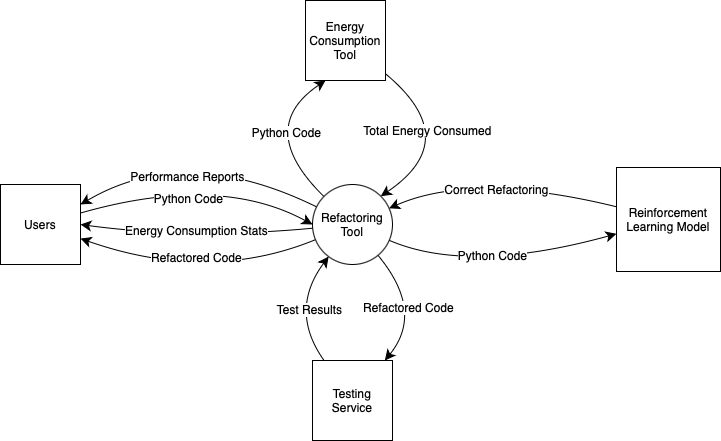
\includegraphics[scale=0.5]{../images/WorkContextModel.png}

\subsection{Work Partitioning}

\scriptsize
\begin{tabular}{ |c|p{2.5cm}|c|c| }
  \hline
  Event \# & Event Name & Input & Output(s) \\
  \hline\hline

  1 & Users submit Python code & Python Code & Refactored Code \\
  2 & Energy Analysis of code & Python Code & Total Energy Consumed \\
  3 & RI Model produces refactoring & Python Code & Correct Refactoring \\
  4 & Testing and Validation of refactored code & Refactored Code & Test Results \\
  5 & Reporting Performance metrics of new code & Refactored Code & Performance Reports \\
  6 & Viewing Energy consumption reports & Refactored Code & Energy Consumption Statistics \\

  \hline
\end{tabular}

\subsection{Specifying a Business Use Case (BUC)}

\subsubsection{Business Use Case Scenario 1}
\textbf{Event Name:} Code Submission \\
\textbf{Input:} Python Code \\
\textbf{Output:} Refactored Code \\
\textbf{Pre-condition:} User uses either GitHub Action or a VS code plugin to submit code to the refactoring tool \\  
\textbf{Scenario:}
    \begin{enumerate}
        \item Refactoring tool receives the Python code
        \item PyJoules is used to store energy consumption data for original Python code submitted
        \item Tool analyzes the code for inefficiencies (PySmells)
        \item Python code is provided to Re-enforcement learning model to find a refactoring
        \item Energy consumption is measured of refactored code and compared to the original data
        \item Refactored code is tested to ensure functionality is maintained from original code
        \item Refactored code is received by the user
    \end{enumerate}
\textbf{Sub Variation: }
    \begin{itemize}
        \item \textit{4a:} If no PySmells identified, then code is returned to the user
        \item \textit{6a:} If energy consumption increases for refactored code, the reinforcement model is asked to find another refactoring
        \item \textit{7a:} If code functionality is not preserved for refactored code, the reinforcement model is asked to find another refactoring
    \end{itemize}

\subsubsection{Business Use Case Scenario 2} 
\textbf{Event Name:} Energy Analysis of Code \\
\textbf{Input:} Python Code \\
\textbf{Output:} Total Energy Consumed \\
\textbf{Pre-condition:} Submission of Python code to the Energy Consumption Tool \\
\textbf{Scenario: } 
\begin{itemize}
    \item \textit{1:} Tool receives Python Code
    \item \textit{2:} Energy consumed is measured during execution
    \item \textit{3:} The analysis results are compiled into a report
    \item \textit{4:} Report of total energy consumed is received by the refactoring tool
\end{itemize}

\subsubsection{Business Use Case Scenario 3} 
\textbf{Event Name:} Reinforcement Learning Model Produces Refactoring \\
\textbf{Input:} Python Code \\
\textbf{Output:} Correct Refactoring \\
\textbf{Pre-condition:} Request for refactored code from the Reinforcement Learning Model \\
\textbf{Scenario: } 
\begin{itemize}
    \item \textit{1:} Model receives Python Code
    \item \textit{2:} Analyze Code for potential refactoring
    \item \textit{3:} Generate suggestions based on previous learning and data
    \item \textit{4:} Implement suggested refactorings
\end{itemize}
\textbf{Sub Variation: }
\begin{itemize}
    \item \textit{2a:} If there are no refactorings found, Model outputs given code back to the refactoring tool 
\end{itemize}

\subsubsection{Business Use Case Scenario 4} 
\textbf{Event Name:} Testing and Validation of Refactored Code \\
\textbf{Input:} Refactored Code \\
\textbf{Output:} Test Results \\
\textbf{Pre-condition:} Energy consumed for refactored code is less than energy consumed for original code \\
\textbf{Scenario: } \\
\begin{itemize}
    \item \textit{1:} Conduct tests on refactored code
    \item \textit{2:} Conduct tests on original code
    \item \textit{3:} Validate results of refactored code to the results of the original code to ensure functionality is intact
    \item \textit{4:} Signal to refactoring tool to send refactored code to user
\end{itemize}
\textbf{Sub Variation: }
\begin{itemize}
    \item \textit{4a:} If functionality is not preserved, signal to the refactoring tool to refactor again
\end{itemize}

\subsubsection{Business Use Case Scenario 5} 
\textbf{Event Name:} Reporting Performance Metrics of New Code \\
\textbf{Input:} Refactored Code \\
\textbf{Output:} Performance Reports\\
\textbf{Pre-condition:} Testing and validation is completed successfully \\
\textbf{Scenario: } \\
\begin{itemize}
    \item \textit{1:} Generate detailed performance report based on testing outcomes
    \item \textit{2:} User receives the performance report
\end{itemize}

\subsubsection{Business Use Case Scenario 6} 
\textbf{Event Name:} Viewing Energy Consumption Reports \\
\textbf{Input:} Refactored Code \\
\textbf{Output:} Energy Consumption Statistics \\
\textbf{Pre-condition:} Testing and validation is completed successfully \\
\textbf{Scenario: } \\
\begin{itemize}
    \item \textit{1:} Comprehensive statistics are compiled from energy analysis data
    \item \textit{2:} Information is compiled in an accessible format for developers to review
\end{itemize}


\section{Business Data Model and Data Dictionary}
\subsection{Business Data Model}
\lips
\subsection{Data Dictionary}
\lips

\section{The Scope of the Product}
\subsection{Product Boundary}
\lips
\subsection{Product Use Case Table}
\lips
\subsection{Individual Product Use Cases (PUC's)}
\lips

\section{Functional Requirements}
\subsection{Functional Requirements}

\begin{enumerate}
  \item \textbf{Requirement:} The tool must accept Python source code files.
  \begin{itemize}[label={}]
      \item \textbf{Fit Criteria:} The tool successfully processes valid Python files without errors and provides feedback for invalid files.
  \end{itemize}
  \item \textbf{Requirement:} The tool must identify specific code smells that can be targeted for energy saving.
  \begin{itemize}[label={}]
      \item \textbf{Fit Criteria:} The tool should be able to detect and report at least 80\% of the follwing code smells using predefined rules or existing linters. Code smells include: Large Class (LC), Long Parameter List (LPL), Long Method (LM), Long Message Chain (LMC), Long Scope Chaining (LSC), Long Base Class List (LBCL), Useless Exception Handling (UEH), Long Lambda Function (LLF), Complex List Comprehension (CLC), Long Element Chain (LEC), Long Ternary Conditional Expression (LTCE).
  \end{itemize}
  \item \textbf{Requirement:} The tool must suggest at least one appropriate refactoring for each detected code smell to decrease energy consumption or indicate that none can be found.
  \begin{itemize}[label={}]
      \item \textbf{Fit Criteria:} The suggested refactored code demonstrates a measurable improvement in energy measured in joules.
  \end{itemize}
  \item \textbf{Requirement:} The tool must implement an algorithm to choose the most optimal refactoring based on measured energy consumption.
  \begin{itemize}[label={}]
      \item \textbf{Fit Criteria:} The algorithm evaluates multiple refactoring options and selects the one that results in the lowest energy consumption for the given code smell.
  \end{itemize}
  \item \textbf{Requirement:} The tool must produce valid refactored python code as output or indicate that no possible refactorings were found.
  \begin{itemize}[label={}]
      \item \textbf{Fit Criteria:} The output code is syntactically correct and adheres to Python standards, validated by an automatic linter.
  \end{itemize}
  \item \textbf{Requirement:} The tool must report to the user any discrepancies between the original and suggested refactored code.
  \begin{itemize}[label={}]
      \item \textbf{Fit Criteria:} Discrepancy reports to user clearly highlight differences in outputs
  \end{itemize}
  \item \textbf{Requirement:} The tool must allow users to input their original test suite as a required argument.
  \begin{itemize}[label={}]
      \item \textbf{Fit Criteria:} Users can specify a path to their test suite, and the tool recognizes and utilizes it for testing the refactored code.
  \end{itemize}
  \item \textbf{Requirement:} The tool must ensure that the original functionality of the code is preserved after refactoring.
  \begin{itemize}[label={}]
      \item \textbf{Fit Criteria:} The tool runs the original test suite against the refactored code, and passes 100\% of the tests.
  \end{itemize}
  \item \textbf{Requirement:} The tool must be compatible with various Python versions and common libraries.
  \begin{itemize}[label={}]
      \item \textbf{Fit Criteria:} The tool operates correctly with the latest two major versions of Python (e.g., Python 3.8 and 3.9) and commonly used libraries.
  \end{itemize}
  \item \textbf{Requirement:} The tool must generate comprehensive reports on detected smells, refactorings applied, energy consumption measurements, and testing results.
  \begin{itemize}[label={}]
      \item \textbf{Fit Criteria:}  Reports are clear, well-structured, and provide actionable insights, with users able to easily understand the results.
  \end{itemize}
  \item \textbf{Requirement:} The tool must provide comprehensive documentation and help resources.
  \begin{itemize}[label={}]
      \item \textbf{Fit Criteria:} Documentation covers installation, usage, and troubleshooting, receiving positive feedback for clarity and completeness from users.
  \end{itemize}
\end{enumerate}

\section{Look and Feel Requirements}
\subsection{Appearance Requirements}
\lips
\subsection{Style Requirements}
\lips

\section{Usability and Humanity Requirements}
\subsection{Ease of Use Requirements}
\begin{enumerate}
  \item \textbf{Requirement:} The tool must have an intuitive user interface that simplifies navigation and functionality.
  \begin{itemize}[label={}]
      \item \textbf{Fit Criteria:}  Users should be able to complete key tasks (e.g., parsing code, configuring settings) within three clicks or less.
  \end{itemize}
  \item \textbf{Requirement:} The tool should provide clear and concise prompts for user input.
  \begin{itemize}[label={}]
      \item \textbf{Fit Criteria:} At least 90\% of test users should report that prompts are straightforward and guide them effectively through the process.
  \end{itemize}
\end{enumerate}
\subsection{Personalization and Internationalization Requirements}
\begin{enumerate}
  \item \textbf{Requirement:}The tool should allow users to customize settings to match their preferences (e.g., refactoring styles, detection sensitivity).
  \begin{itemize}[label={}]
      \item \textbf{Fit Criteria:}  Users should be able to save and load custom configurations easily.
  \end{itemize}
  \item \textbf{Requirement:} User guide must be available in French and English.
  \begin{itemize}[label={}]
      \item \textbf{Fit Criteria:} French and english installation and use instructions available.
  \end{itemize} 
\end{enumerate}
\subsection{Learning Requirements}
\begin{enumerate}
  \item \textbf{Requirement:} The tool must have an availible youtube video demonstrating installation.
  \begin{itemize}[label={}]
      \item \textbf{Fit Criteria:}  Youtube video present and easily accessible
  \end{itemize}
  \item \textbf{Requirement:} The tool should provide context-sensitive help that offers assistance based on the current user actions.
  \begin{itemize}[label={}]
      \item \textbf{Fit Criteria:} Help resources should be accessible within 1-3 clicks.
  \end{itemize}
\end{enumerate}
\subsection{Understandability and Politeness Requirements}
\begin{enumerate}
  \item \textbf{Requirement:} The tool should communicate errors and issues politely and constructively.
  \begin{itemize}[label={}]
      \item \textbf{Fit Criteria:} User feedback should reflect that at least 80\% of users perceive error messages as helpful and courteous, rather than frustrating or vague.
  \end{itemize}
  \item \textbf{Requirement:} The tool should provide context-sensitive help that offers assistance based on the current user actions.
  \begin{itemize}[label={}]
      \item \textbf{Fit Criteria:} Help resources should be accessible within 1-3 clicks.
  \end{itemize}
\end{enumerate}
\subsection{Accessibility Requirements}
\begin{enumerate}
  \item \textbf{Requirement:} The tool should provide high-contrast color themes to improve visibility for users with visual impairments.
  \begin{itemize}[label={}]
      \item \textbf{Fit Criteria:} Users should have access to at least 1 high contrast theme.
  \end{itemize}
  \item \textbf{Requirement:} The tool should offer audio cues for important actions and alerts to assist users with use and navigation.
  \begin{itemize}[label={}]
      \item \textbf{Fit Criteria:} At least 70\% of users should report that the audio cues enhance their understanding of important notifications or actions.
  \end{itemize}
\end{enumerate}

\section{Performance Requirements}
\subsection{Speed and Latency Requirements}
\begin{enumerate}
  \item \textbf{Requirement:} The tool must analyze and detect code smells in the input code within a reasonable time frame.
  \begin{itemize}[label={}]
      \item \textbf{Fit Criteria:} The tool should complete the analysis for files up to 1,000 lines of code in under 5 seconds, and for files up to 10,000 lines in under 30 seconds.
  \end{itemize}
  \item \textbf{Requirement:} The refactoring process must be executed efficiently without noticeable delays.
  \begin{itemize}[label={}]
      \item \textbf{Fit Criteria:}  The tool should refactor the code and generate output in under 10 seconds for small to medium-sized files (up to 5,000 lines).
  \end{itemize}
\end{enumerate}

\subsection{Safety-Critical Requirements}
\begin{enumerate}
  \item \textbf{Requirement:} The tool must ensure that no runtime errors are introduced in the refactored code that could result in data loss or system failures.
  \begin{itemize}[label={}]
      \item \textbf{Fit Criteria:} The tool should pass all tests from the user-provided test suite after refactoring, confirming that the original functionality remains intact. The output code is syntactically correct and adheres to Python standards, validated by an automatic linter.
  \end{itemize}
\end{enumerate}

\subsection{Precision or Accuracy Requirements}
\begin{enumerate}
  \item \textbf{Requirement:} The tool must reliably identify code smells with minimal false positives and negatives.
  \begin{itemize}[label={}]
      \item \textbf{Fit Criteria:} Detection accuracy should exceed 90\% when validated against a set of known cases.
  \end{itemize}
  \item \textbf{Requirement:} The tool must maintain the functionality of the original provided code in all its reccommended refactorings.
  \begin{itemize}[label={}]
      \item \textbf{Fit Criteria:} The tool should pass all tests from the user-provided test suite after refactoring, confirming that the original functionality remains intact.
  \end{itemize}
  \item \textbf{Requirement:} The tool must produce valid refactored python code as output or indicate that no possible refactorings were found.
  \begin{itemize}[label={}]
      \item \textbf{Fit Criteria:} The output code is syntactically correct and adheres to Python standards, validated by an automatic linter.
  \end{itemize}
\end{enumerate}
\subsection{Robustness or Fault-Tolerance Requirements}
\begin{enumerate}
  \item \textbf{Requirement:} The tool should gracefully handle unexpected inputs, such as invalid code or non-Python files.
  \begin{itemize}[label={}]
      \item \textbf{Fit Criteria:} The tool should provide clear error messages and recover from input errors without crashing, ensuring stability.
  \end{itemize}
  \item \textbf{Requirement:} The tool must have fallback options if a specific refactoring attempt fails.
  \begin{itemize}[label={}]
      \item \textbf{Fit Criteria:} In the event of a failed refactoring, the tool should log the error and propose alternative refactorings without stopping the process.
  \end{itemize}
\end{enumerate}
\subsection{Capacity Requirements}
\begin{enumerate}
  \item \textbf{Requirement:} The tool should efficiently manage large codebases.
  \begin{itemize}[label={}]
      \item \textbf{Fit Criteria:} The tool must process projects with up to 100,000 lines of code within 2 minutes, maintaining performance standards.
  \end{itemize}
\end{enumerate}
\subsection{Scalability or Extensibility Requirements}
\begin{enumerate}
  \item \textbf{Requirement:} The tool should be designed to allow easy addition of new code smells and refactoring methods in future updates.
  \begin{itemize}[label={}]
      \item \textbf{Fit Criteria:}  New code smells or refactorings can be incorporated with minimal changes to existing code, ensuring that current functionality remains intact.
  \end{itemize}
\end{enumerate}
\subsection{Longevity Requirements}
\begin{enumerate}
  \item \textbf{Requirement:} The tool should be maintainable and adaptable to future versions of Python and changing coding standards.
  \begin{itemize}[label={}]
      \item \textbf{Fit Criteria:} The codebase should be well-documented and modular, facilitating updates with minimal effort.
  \end{itemize}
\end{enumerate}

\section{Operational and Environmental Requirements}
% \begin{enumerate}[{OER-WE}1. ]
	% \item \emph{}\\
  %   {\bf Rationale:} \\
  %   {\bf Fit Criterion:}  
% \end{enumerate}
\subsection{Expected Physical Environment}

\begin{enumerate}[label=OER-EP \arabic*., wide=0pt, leftmargin=*]
	\item \emph{The product shall be used in temperatures ranging from \SI{10}{\celsius} - \SI{35}{\celsius}.}\\
    {\bf Rationale:} A computer's safe operating range is \SI{10}{\celsius} - \SI{35}{\celsius} ~\citep{PCTemp}. If the computer doesn't work then it is not possible to use the refactoring library. \\
    {\bf Fit Criterion:} The computer turns on, and no temperature warning is issued.
  \item \emph{The product shall be used in proximity to a stable power supply.}\\
  {\bf Rationale:} As a coding library, the product depends on the continuing operation of the computer system it is used on. Should the computer lose power, the refactoring library will see its processes halted. \\
  {\bf Fit Criterion:} The computer is connected to a power outlet or the computer possesses charge on its battery. 
\end{enumerate}

\subsection{Wider Environment Requirements}
\begin{enumerate}[label=OER-WE \arabic*., wide=0pt, leftmargin=*]
	\item \emph{The system must align with widely used emissions standards (e.g., GRI 305, GHG, ISO 14064) ~\citep{GHG,ISO14064,GRI305}.}\\
    {\bf Rationale:} Providing metrics tailored to these standards, makes the library reporting tool more attractive to users part of companies looking to reduce their ecological footprint. \\
    {\bf Fit Criterion:} The emissions tracked by the standards are present in the reported metrics.  
\end{enumerate}

\subsection{Requirements for Interfacing with Adjacent Systems}
\begin{enumerate}[label=OER-IAS \arabic*., wide=0pt, leftmargin=*]
	\item \emph{The refactoring library must provide integration capabilities with GitHub Actions.}\\
    {\bf Rationale:} This will allow the automation of the refactoring process within existing workflows to ensure that energy-efficient practices are consistently applied during continuous integration.\\
    {\bf Fit Criterion:} The library is available to use via GitHub Actions when writing workflows.
  \item \emph{The library should be compatible with the Visual Studio Code (VSCode) IDE.}\\
    {\bf Rationale:} Developers will be able to refactor code easily without leaving their working environment, therefore enhancing the accessibility and usability of the library.\\
    {\bf Fit Criterion:} An extension is available for installation in VSCode marketplace.
  \item \emph{The library should support importing existing codebases and exporting refactored code and energy savings reports in standard formats (e.g., JSON, XML)}\\
    {\bf Rationale:} This ensures that users can easily integrate the library into their existing workflows without significant disruption.\\
    {\bf Fit Criterion:} Developers are able to refactor existing codebases and view relevant metrics.
\end{enumerate}

\subsection{Productization Requirements}
\begin{enumerate}[label=OER-PR \arabic*., wide=0pt, leftmargin=*]
	\item \emph{The library shall be package with PIP and made available to python users through the public package manager.}\\
    {\bf Rationale:} As a widely used package manager, PIP will be able to distribute the library to any users that wish to use it.\\
    {\bf Fit Criterion:} Users are able to install the library using \texttt{pip install}. 
\end{enumerate}

\subsection{Release Requirements}
\begin{enumerate}[label=OER-RL \arabic*., wide=0pt, leftmargin=*]
	\item \emph{All core functionalities specified in the requirements must be implemented and tested, including energy consumption measurement, automated refactoring, and reporting features.}\\
    {\bf Rationale:} This will ensures that the library delivers the promised capabilities to users.\\
    {\bf Fit Criterion:} Follows the steps outlined in the Verification and Validation (V\&V) plan.  
  \item \emph{The library must be ready for release by March 17th, 2025.}\\
    {\bf Rationale:} The library must be ready for final demonstration as a requirement of the McMaster University SFRWENG 4G06 Capstone course.\\
    {\bf Fit Criterion:} The project is ready for the final demonstration of the appointed date.
\end{enumerate}

\section{Maintainability and Support Requirements}
\subsection{Maintenance Requirements}
\begin{enumerate}
  \item \textbf{Requirement:} The tool must allow new refactoring techniques to be added within one week of identification.
     \begin{itemize}
         \item \textbf{Rationale:} Rapid integration of new techniques ensures the tool remains up-to-date with evolving best practices in energy-efficient coding.
         \item \textbf{Fit Criteria:} Developers can integrate new refactoring methods into the tool, and they are fully operational within seven days.
     \end{itemize}
     
  \item \textbf{Requirement:} The tool must be maintainable by developers who are not the original creators.
     \begin{itemize}
         \item \textbf{Rationale:} Ensuring that new developers can easily understand and modify the system reduces dependency on original developers and facilitates long-term maintenance.
         \item \textbf{Fit Criteria:} Comprehensive documentation is available, including setup guides and code comments, allowing new developers to understand and modify the system within two days.
     \end{itemize}
     
  \item \textbf{Requirement:} The tool must allow for easy rollback of updates in case of errors.
     \begin{itemize}
         \item \textbf{Rationale:} Quick rollback capabilities minimize downtime and user disruption in case an update introduces issues.
         \item \textbf{Fit Criteria:} Any update can be reverted with minimal effort, ensuring the system returns to a stable state within one hour.
     \end{itemize}
     
  \item \textbf{Requirement:} The tool must provide automated testing for all refactoring functions.
     \begin{itemize}
         \item \textbf{Rationale:} Automated testing ensures that changes do not introduce new bugs, maintaining the reliability and stability of the tool.
         \item \textbf{Fit Criteria:} All refactoring methods have associated unit tests that run automatically with each code change, ensuring 80\% code coverage.
     \end{itemize}
     
  \item \textbf{Requirement:} Each version of the library must maintain compatibility with the current releases of external libraries during its development phase. .
     \begin{itemize}
         \item \textbf{Rationale:} Keeping external libraries up-to-date ensures compatibility and leverages improvements or security patches provided by library maintainers.
         \item \textbf{Fit Criteria:} The system successfully integrates updates from external libraries without breaking existing functionality.
     \end{itemize}
  
  \end{enumerate}

\subsection{Supportability Requirements}
\begin{enumerate}
  \item \textbf{Requirement:} The tool must offer bilingual support for help documentation.
  \begin{itemize}
      \item \textbf{Rationale:} Bilingual support ensures that users from different regions can understand and use the tool effectively, increasing its accessibility.
      \item \textbf{Fit Criteria:} Help documentation is available in both major languages, English and French.
  \end{itemize}
  
\end{enumerate}

\subsection{Adaptability Requirements}
Not applicable in this project currently

\section{Security Requirements}
\subsection{Access Requirements}
\lips
\subsection{Integrity Requirements}
\lips
\subsection{Privacy Requirements}
\lips
\subsection{Audit Requirements}
\lips
\subsection{Immunity Requirements}
\lips

\section{Cultural Requirements}
\subsection{Cultural Requirements}
\begin{enumerate}
  \item \textbf{Requirement:} The tool must avoid using colors or symbols that could be culturally sensitive or offensive.
  \begin{itemize}
      \item \textbf{Rationale:}  Ensuring cultural sensitivity in design helps avoid alienating or offending users from diverse backgrounds, which is critical for global acceptance and usability.
      \item \textbf{Fit Criteria:} Conduct a cultural review to ensure that all icons and colors used in the tool are neutral and universally acceptable.
  \end{itemize}
  
  \item \textbf{Requirement:} The tool must support both metric and imperial measurement units.
  \begin{itemize}
      \item \textbf{Rationale:} Users have different preferences and standards for measurement units. Supporting both metric and imperial units ensures accessibility and ease of use for a global audience.
      \item \textbf{Fit Criteria:} Users can toggle between metric and imperial units for any measurements related to energy consumption.
  \end{itemize}   
  
  \item \textbf{Requirement:} The tool must not include content that could be considered culturally insensitive.
  \begin{itemize}
      \item \textbf{Rationale:} Avoiding culturally insensitive content ensures that the tool is respectful and inclusive, fostering a positive user experience across different cultures.
      \item \textbf{Fit Criteria:} A cultural sensitivity review is conducted to ensure all content is appropriate for a global audience.
  \end{itemize}

\end{enumerate}

\section{Compliance Requirements}
\subsection{Legal Requirements}
\lips
\subsection{Standards Compliance Requirements}
\lips

\section{Open Issues}
\lips

\section{Off-the-Shelf Solutions}
\subsection{Ready-Made Products}

\begin{itemize}
  \item \textbf{Pylint:} A widely used static code analysis tool that detects various code smells in Python. It can be integrated into the refactoring tool to help identify inefficiencies in the code.
  \item \textbf{Flake8:} Linter that combines checks for style guide enforcement and code quality. Flake8 can assist in maintaining code standards while the tool focuses on energy efficiency.
  \item \textbf{PyJoule:} A tool for measuring the energy consumption of Python code. This product can provide essential data to evaluate the impact of refactorings on energy usage.
\end{itemize}

\subsection{Reusable Components}
\begin{itemize}
  \item \textbf{Rope:} A library for Python that provides automated refactoring capabilities, helping streamline the process of improving code quality.
\end{itemize}
\subsection{Products That Can Be Copied}
\begin{itemize}
  \item \textbf{SonarQube:} An open-source platform designed for continuous inspection of code quality. It helps developers manage code quality and security by analyzing source code to identify potential issues.Its architecture and methods for detecting code smells could be adapted to focus specifically on energy efficiency. 
\end{itemize}

\section{New Problems}
\subsection{Effects on the Current Environment}
The introduction of the energy efficiency refactoring tool may lead to several changes in the current development environment. These effects include:
\begin{enumerate}
  \item The tool temporarily increasing CPU and memory usage while running. The tool aims to optimize energy efficency in code however it takes energy to run - in large codebases this could be significant energy and impact the performance of other applications running concurrently. 
  \item The tool may have it's own dependencies that now need to be included in the app or installed into the current system. Think Pysmells, Pyjoule etc.
\end{enumerate}

\subsection{Effects on the Installed Systems}
\begin{enumerate}
  \item Existing systems may need to be evaluated for compatibility with the new tool. Older versions of python or other needed dependencies may not support the tool.
  \item The refactoring process could lead to variations in the performance of existing applications
  \item As the tool updates existing code, thorough testing will be needed to ensure everything still works correctly. This may require more effort from QA teams and additional time and resources to check the updated code.
\end{enumerate}

\subsection{Potential User Problems}
\begin{enumerate}
  \item Users may face difficulties in understanding how to effectively utilize the tool, particularly if they are not familiar with concepts like code smells and refactoring techniques. This learning curve may lead to initial frustration or reduced productivity.
  \item Some users may be resistant to adopting new tools or processes, particularly if they perceive the existing workflows as sufficient. This resistance could hinder the tool's successful implementation and limit its overall effectiveness.
  \item Users may misinterpret the output reports generated by the tool, such as energy savings or performance metrics. If users do not fully understand how to interpret these results, it could lead to incorrect conclusions about the tool's impact on their code.
  \item There is a risk that users might become overly reliant on the tool for refactoring without fully understanding the underlying principles. This could result in poor coding practices if users do not engage in thoughtful analysis of the suggested changes.
\end{enumerate}
\subsection{Limitations in the Anticipated Implementation Environment That May
Inhibit the New Product}
\begin{enumerate}
  \item \textbf{Limited Computational Resources:} Environments with restricted computational power may face challenges when running the tool, especially for large codebases. Limited resources could result in longer processing times or failures during analysis and refactoring.
  \item \textbf{Lack of Test Coverage:} If existing codebases lack comprehensive test suites, validating the functionality of refactored code may become challenging. Without adequate tests, it will be difficult to ensure that the tool's changes do not introduce new issues.
\end{enumerate}
\subsection{Follow-Up Problems}
\begin{enumerate}
  \item \textbf{Ongoing Maintenance:} The tool will need regular updates to stay compatible with new programming languages or standards, adding to the workload.
  \item \textbf{Performance Trade-offs:} Users may find that while some refactorings improve energy efficiency, they could negatively impact other performance metrics, such as execution speed.
\end{enumerate}
\section{Tasks}
\subsection{Project Planning}
\begin{itemize}
 
  \item \textbf{Development Approach}
  The team will use an agile development approach with the following high-level process:
  \begin{enumerate}
    \item Initial requirements gathering and product backlog creation
    \item Sprint planning and execution
    \item Regular testing and quality assurance
    \item Stakeholder reviews and feedback
    \item Iterative refinement
    \item Release planning and deployment
  \end{enumerate}
  
 \item \textbf{Key Tasks}
  \begin{itemize}
    \item Form cross-functional development team (already completed) 
    \item Create initial product backlog and prioritize features
    \item Set up development environments and tools
    \item Establish CI/CD pipeline using GitHub Actions
    \item Develop core functionality:
      \begin{itemize}
        \item Determine code smells to address for energy saving
        \item Implement code smell detection
        \item Develop appropriate refactorings for detected smells
        \item Measure energy consumption before and after refactoring
        \item Ensure original code functionality is preserved
      \end{itemize}
    \item Build out additional features iteratively
    \item Conduct regular testing (unit, integration, user acceptance)
    \item Refine based on stakeholder feedback
    \item Present final solution to stakeholders

  \end{itemize}
  \item \textbf{Timeline Estimate}
    \begin{itemize}
        \item Requirements Document (Revision 0): October 9th, 2024
        \item Hazard Analysis (Revision 0): October 23rd, 2024
        \item Verification \& Validation Plan (Revision 0): November 1st, 2024
        \item Proof of Concept: November 11th-22nd, 2024
        \item Design Document (Revision 0): January 15th, 2025
        \item Project Demo (Revision 0): February 3rd-14th, 2025
        \item Final Demonstration: March 17th-30th, 2025
        \item Final Documentation: April 2nd, 2025
        \item Capstone EXPO: TBD
    \end{itemize}
    
  \item \textbf{Resource Estimates}
  The team consists of 5 members who will all function as developers, sharing responsibilities for creating issues, coding, testing, and documentation.

  \item \textbf{Key Consideration}
    \begin{itemize}
        \item Data migration may be necessary for existing systems
        \item A phased development approach will help minimize major setbacks
        \item Regular stakeholder involvement will ensure alignment with business needs
    \end{itemize}

  \item \textbf{Documentation Process}
    \begin{itemize}
        \item Pull changes from \texttt{docs} (epic documentation branch)
        \item Create working branch with format [main contributor name]/[descriptive topic]
        \item Commit changes with descriptive names
        \item Create unit tests for changes
        \item Create pull request to merge changes into epic branch
        \item Wait for all tests run with GitHub Actions to pass
        \item Wait for at least two approvals from teammates
        \item Merge changes into target branch
    \end{itemize}
  
\end{itemize}

By following this agile approach and development process, the team aims to deliver a high-quality product iteratively while maintaining flexibility to adapt to changing requirements

\subsection{Planning of the Development Phases}

The planning of the development phases is based on the deliverables submissions as follows:

\begin{enumerate}

    \item \textbf{Requirements Phase}
    \begin{itemize}
        \item Deliverable: Requirements Document (Revision 0)
        \item Due Date: October 9th, 2024
    \end{itemize}
    
    \item \textbf{Risk Assessment Phase}
    \begin{itemize}
        \item Deliverable: Hazard Analysis (Revision 0)
        \item Due Date: October 23rd, 2024
    \end{itemize}
    
    \item \textbf{Verification and Validation Planning}
    \begin{itemize}
        \item Deliverable: Verification \& Validation Plan (Revision 0)
        \item Due Date: November 1st, 2024
    \end{itemize}
    
    \item \textbf{Proof of Concept Implementation}
    \begin{itemize}
        \item Period: November 11th-22nd, 2024
    \end{itemize}
    
    \item \textbf{Design Phase}
    \begin{itemize}
        \item Deliverable: Design Document (Revision 0)
        \item Due Date: January 15th, 2025
    \end{itemize}
    
    \item \textbf{Initial Implementation and Demo}
    \begin{itemize}
        \item Deliverable: Project Demo (Revision 0)
        \item Period: February 3rd-14th, 2025
    \end{itemize}
    
    \item \textbf{Final Implementation and Testing}
    \begin{itemize}
        \item Deliverable: Final Demonstration
        \item Period: March 17th-30th, 2025
    \end{itemize}
    
    \item \textbf{Project Closure}
    \begin{itemize}
        \item Deliverable: Final Documentation
        \item Due Date: April 2nd, 2025
    \end{itemize}
    
    \item \textbf{Project Presentation}
    \begin{itemize}
        \item Event: Capstone EXPO
        \item Date: TBD
    \end{itemize}
\end{enumerate}


\section{Migration to the New Product}
\subsection{Requirements for Migration to the New Product}
\lips
\subsection{Data That Has to be Modified or Translated for the New System}
\lips

\section{Costs}
\lips
\section{User Documentation and Training}
\subsection{User Documentation Requirements}
\begin{enumerate}
  \item \textbf{User Manual}
  \begin{itemize}
      \item \textbf{Purpose:} Provide comprehensive guidance on how to use the refactoring library
      \item \textbf{Target Audience:} Software developers integrating the library into their projects
      \item \textbf{Content:} Installation instructions, API reference, usage examples, and best practices
  \end{itemize}

  \item \textbf{Technical Specification}
  \begin{itemize}
      \item \textbf{Purpose:} Detail the library's architecture, algorithms, and integration points
      \item \textbf{Target Audience:} Technical leads and architects evaluating the library
      \item \textbf{Content:} System design, performance characteristics, and technical limitations
  \end{itemize}

  \item \textbf{Quick Start Guide}
  \begin{itemize}
      \item \textbf{Purpose:} Enable rapid adoption and basic usage of the library
      \item \textbf{Target Audience:} New users looking to quickly implement the library
      \item \textbf{Content:} Concise setup instructions and simple usage examples
  \end{itemize}
\end{enumerate}

\subsection{Training Requirements}
Not Applicable.

\section{Waiting Room}
\lips

\section{Ideas for Solution}
\lips

\newpage{}
\section*{Appendix --- Reflection}

The information in this section will be used to evaluate the team members on the
graduate attribute of Lifelong Learning.  Please answer the following questions:

\begin{enumerate}
  \item What knowledge and skills will the team collectively need to acquire to
  successfully complete this capstone project?  Examples of possible knowledge
  to acquire include domain specific knowledge from the domain of your
  application, or software engineering knowledge, mechatronics knowledge or
  computer science knowledge.  Skills may be related to technology, or writing,
  or presentation, or team management, etc.  You should look to identify at
  least one item for each team member.
  \item For each of the knowledge areas and skills identified in the previous
  question, what are at least two approaches to acquiring the knowledge or
  mastering the skill?  Of the identified approaches, which will each team
  member pursue, and why did they make this choice?
\end{enumerate}

\subsubsection*{Mya Hussain Reflection}
\begin{enumerate}
  \item \textit{What knowledge and skills will the team collectively need to acquire to
  successfully complete this capstone project?}

    \begin{itemize}
      \item Understanding of Python's performance characteristics and common code smells
      \item Experience in using libraries like rope for automated refactoring and familiarity with integrating linters such as Pylint or Flake8 into the development workflow.
      \item Ability to develop algorithms that analyze and compare different refactoring strategies, using tools like PyJoule for energy profiling.
      \item  Proficiency in JavaScript or TypeScript, as most VS Code extensions are developed using these languages.
    \end{itemize}
 
\end{enumerate}

\bibliographystyle {plainnat}
\bibliography{../../refs/References}

\end{document}

